\section{Product perspective}

The project aims to build a system that manage the users’ booking without wasting time while they're waiting their own turn outside the market. 
\par
An other important aspect is that the application should be for multiple market. Each user at the beginning will choose the market in which are going to go grocery shopping.\\
Indeed, we think that it had better that more markets adopt this system, due to increase safety in social distance.
\par
For a \textbf{Reservation} the system provides User infomation about queue's dynamic in real time (i.e the number of people ahead). 
To do this, the application should try, in the best way, to estimate the time that the customers will spend in the market, in order to notify in advance users who are waiting their own turn outside. 



In addition Users have to indicate how long the shopping time will be, putting potentially the \textbf{size} of the expenditure. This could be \textit{small}, \textit{medium} or \textit{large}.
\\
The application analyses the customers’ statistics and computes the average shopping time.
The calculation considers the time range between the moments in which the User goes in and out.  
In this way, the other customers in queue will be notified as soon as it's the right time to leave and reach the market in time due to the queue's congestion and his position.  

\par
Moreover, it's possible to book a visit choosing the date and the schedule in advance choosing the \textbf{Visit} option. 
\\
The timetable will be splitted into 30 minutes slots, and customers will choose which they want among the free ones. \par

In addition each market will provide customer, who don't have the application or even a smartphone, a toll-free number in order to make an appointment.
%book a visit or reserve a seat in a virtual queue 
This would be easy-manageble because for each market a \textbf{Receptionist} handles the booking and advises the customers with the best shopping option. %as clients' necessary. 
At the beginning, the user will be sign up for booking: so the receptionist will ask the required data from him and will create a customer profile in the system.

The user can also manage (either \textit{delete} or \textit{postpone}), in a later moment, his reservation by calling the same number of the registration.



An \textbf{SMS} will provide:
\begin{itemize}
\item the time in which he have to access to the market;
\item the identification string which will be submitted at the entrance;
\end{itemize}

Once the user finished his shopping, he will scan the code at the exit to open the doors.
\bigskip
In the UML diagram below will be list the main classes in order to understand how the whole system works.

\par 
\bigskip
\bigskip
\begin{figure}[H]
  \label{fig:UML}
  \centering
  \makebox[\linewidth]{
    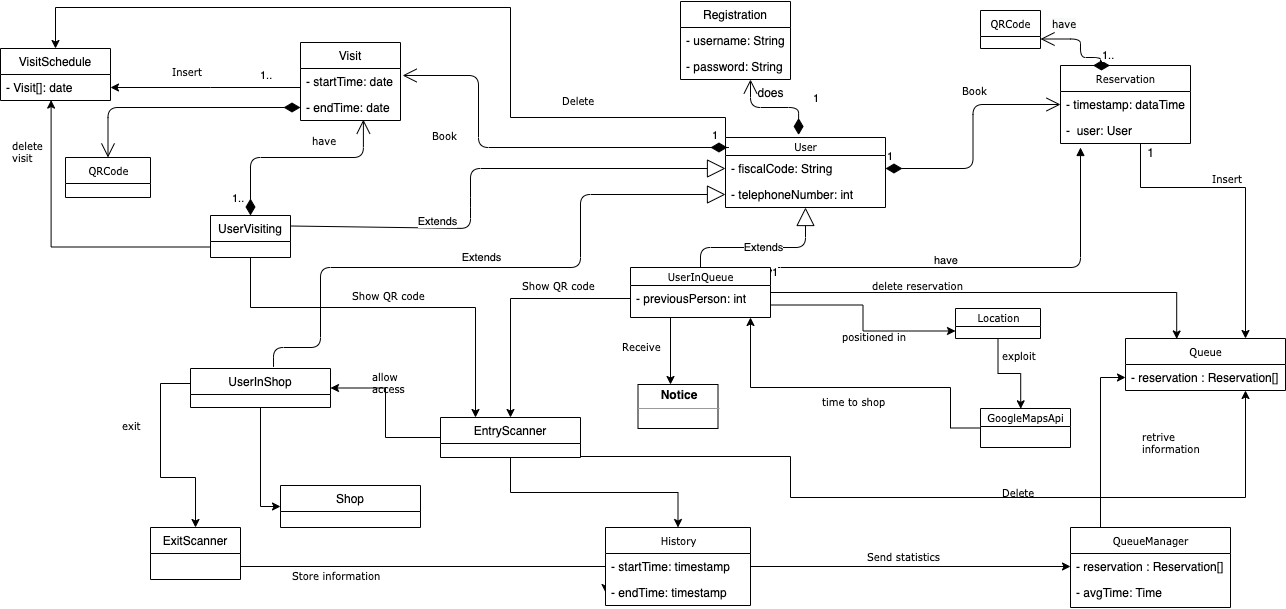
\includegraphics[scale=0.35]{diagrams/UML_simple.png}}
  \caption{Class diagram with UML}
\end{figure}



\par 
\medskip
As we can see from the class diagram in figure~\ref{fig:UML}, the User can book once or a Visit or a Reservation.
In both cases will be provide him a QRcode, which will be submitted to enter in the market. 
If the the User decided to undo his Reservation in the queue could do it by making a cancellation from the application. 
\par
\medskip

In addition the system will notice to Smart User through a notification  when it's almost his turn.

Now we will analyze the interaction between the User and the system, in order to understand possible criticities.
\par 
\bigskip

\begin{figure}[h]
  \caption{State diagram of the Reservation in the queue}
  \label{fig:Reservation}
  \centering
  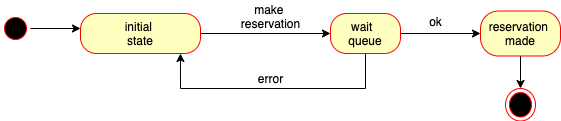
\includegraphics[width=0.8\textwidth, height=0.2\textwidth]{diagrams/2-reservation.png}

\end{figure}
\par 
\medskip

In the first state diagram (figure~\ref{fig:Reservation}) it can be osserved how a generic User can make a reservation thorugh the system. It's sufficient making this action to be added in queue to enter in the market.
\\If something goes wrong the User will be redirect to the initial state.
\\Usually the system reject the request if the market is next to closure (or for logistic problem).

\par 
\medskip

\begin{figure}[h]
  \caption{State diagram of booking a Visit}
  \label{fig:Visit}
  \centering
  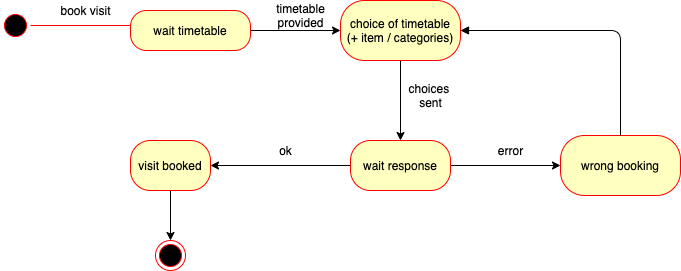
\includegraphics[width=0.8\textwidth, height=0.4\textwidth]{diagrams/2-visit.png}
\end{figure}

\par 
\medskip

Instead, the figure~\ref{fig:Visit} explains how to book a visit in the market. Once the timetable is provided, the generic user have to select the range time of the visit and the size bag.
\\
If the choice made by the user is wrong (i.e timetable's slot full or market closed), the system notify him; the User will try again until his choice is correct.
\par 
\medskip


\section{Product functions}
\subsection{Queue manager}
This is one of the most important function that our system must provide because it must avoid the users waiting too much their turn in the case of a wrong use of notifications. 
In fact, it have to foresee, through statistics from users’ information, the correct time in which the users will enter in the market. This can be done thanks to the notifications sent to the user.
It will also have to decide whether to accept or refuse an appointment, depending on the shop closing time and the number of people in queue. 



To anticipated the unexpected, the system will use a grace.
Let us assume that the maximum number of Users into the market is 100. Well, the system will provide only 90 users.
\\
The remaining 10 will be used only for emergency or in the time period in which the customer will enter or exit from the market.
This grace will be a usefull resource for the system because it can manage non-deterministic event, like user's shopping time.
\\%, which is a stochastic prediction.
The system will determine the average shopping time according to the information who the user enter during his booking.
\par
In particular accuracy of the computation depends on the quality of User's data.
In this way, when the shopping time will be near to the average shopping time, the system will notice the first user in queue to reach the supermarket.  
Our goal is to monitor the User's influx and to keep it under critical boundary (more or less 95\%). Therefore this could be possibile by flowing slowly the virtual queue.
\par
\subsection{Data Collection}
The \textit{Data Collection} is essential for the correct regulation of users' flow, because it will have to provide precise dates according to client’s information. 
Therefore, the system will have to ask clients precise information according to keep useful knowledge for estimating the shopping time into the supermarket, without violating users’ privacy. 
\\
In order to achieve this goal, it needs to oblige the user to register himself in the system and to check the item to allow the processing of his personal data, necessary to reserve virtually the seat in the queue.
\\
One of the possible information asked could be the duration of the expenses. This will be used, with the entry time, to track the number of user inside the market who is finishing. Then, will be possibile to notify in advance users in queue about the closeness of their turn.

\section{User characteristics}
We distinguish the actors into our application based on actions and interactions with the external world:

\begin{itemize}
\item \textit{User}: he’s a client who has signed in the system and he can book a visit or take his queue number.
\item \textit{User in Queue}: he’s a User who has taken his own turn in queue and he’s waiting for the system notification
\item \textit{User visiting}: he’s a User who has booked a visit and he’s still waiting for entering into the supermarket.
\item \textit{User in market}: he’s a client who has taken his own queue ticket or he has booked a visit. After that he is arrived at the supermarket, he has scanned the QR code and he has entered into the shop.
\end{itemize}


\section{Assumptions, dependencies and constraints}
\subsection{Assumptions}
\begin{description}
    \item[D1] The system can delete the Reservation when the Smart User accumulates a delay to reach the market greater than 10 minutes; 
    \item[D2] The system can delete the Reservation the Mobile User accumulates a delay to reach the market greater than 15 minutes; 
    \item[D3] The system handles the threshold number of Users allowed in the market;
    \item[D4] The Smart User have to be connected to Internet through Wi-Fi/Cellular network;
    \item[D5] The Mobile User have to be connected to his own mobile operator;
    \item[D6] A Visit is associated to a Date and a period of time (start/end time);
    \item[D7] A Booking is associated to one and only one QRCode;
    \item[D8] User must have one and only one Visit activated;
    \item[D9] User must have one and only one Reservation activated;
    \item[D10] A Booking belongs to one and only one User;
    \item[D11] The time  of entrance plus the duration of the grocery shopping mustn’t exceed the time in which the market will be closed; 
    \item[D12] In each Date and Slot Time must contain at most N ;
    \item[D13] An User mustn’t have a Reservation and a Visit active and submitted at the same time;
    \item[D14] Smart User must be recognized at the entrance by an employee by his identity document;   
\end{description}

